\documentclass[12pt,letterpaper]{article}

\usepackage{bargar}
\usepackage{euler}
\usepackage{amsmath}
\usepackage{pdfpages}
\usepackage{graphicx}
\usepackage{amsmath}

\assignment{Heat Exchanger Design}
\student{Joshua Holbrook}
\duedate{April 23\textsuperscript{rd} 2010}
\coursename{Thermal Systems Lab}
\coursenumber{ME 415}

\begin{document}
\sffamily

\section{Introduction}

stuff

\section{Methodology}

The basis of this analysis is the Log Mean Temperature Difference method, or LMTD method, which relies on the relation in equations \ref{eq:lmtd}, \ref{eq:cpdt} and \ref{eq:lmtd_def}, where \(T_i\) is the ith temperature, \(A_s\) is the surface area over which heat transfer is occuring, and \(U\) is the total heat transfer coefficient for the apparatus.

\begin{align}
\label{eq:lmtd}
\dot{Q} &= UA_s F(\textrm{LMTD})\\
\label{eq:cpdt}
        &= \dot{m}c_P \Delta T_{\textrm{hot}}
\end{align}

\begin{equation}
\label{eq:lmtd_def}
\textrm{LMTD} = 
\frac{ (T_{\textrm{hot, in}} - T_{\textrm{cold, out}} ) -
       (T_{\textrm{cold, in}} - T_{\textrm{hot, out}})
     }{
\log\left( 
    (T_{\textrm{hot, in}} - T_{\textrm{cold, out}} )
    \middle/ 
    (T_{\textrm{cold, in}} - T_{\textrm{hot, out}}) 
    \right) }
\end{equation}

In this case, the LMTD is defined as with the case of a counter-flow heat exchanger.  In this analysis, however, I am assuming a cross-flow heat exchanger, which requires a correction factor \(F\) to be used. This correction factor is a function of all four inlet/outlet temperatures, as well as the particular geometry of the heat exchanger.  For this analysis, the relations encoded in Cengel's Heat and Mass Transfer's graphs were used, assuming unmixed flow. \marginpar{pictures?}

From the constraints and assumptions for this heat exchanger design, both the LMTD and \(F\) may be found.  In addition, based on the constraints for the hot side of the heat exchanger, \(\dot{Q}\) may also be calculated. With these pieces of information, we may find what the product \(UA_s\) must be in order to meet the constraints for the heat exchanger design. 

The tough part, naturally, is finding good values for \(U\) and \(A_s\). \(A_s\) is a function of the heat exchanger's geometry.  \(U\) relates to the geometry and the materials involved as in equation \ref{eq:U}, for the case of a brazed plate heat exchanger.

\begin{equation}
\label{eq:U}
U = \left(\frac{2}{h} + \frac{A_{s, \textrm{plate}} t_{\textrm{plate}}}{k_{\textrm{solid}}} \right)^{-1}
\end{equation}

This means that not only must \(A_s\) be known, but so must the thickness of the plates, the material the exchanger is made of, and the convective heat transfer coefficient across the plates, which is in turn a function of the geometry of the heat exchanger, the material properties of the fluid, and the velocity of the fluids through the exchanger.

For this design, I decided to start with pre-fabricated plates designed for brased plate heat exchangers. This gives a good starting point for the design of the heat exchanger, removing a lot of the design variables, while still requiring the basic calculations required to actually design a heat exchanger. Moreover, while the plates might be already-designed in real life, specifications on them detailed enough to base the entire design are not easily-obtained. Therefore, basic released knowledge of plate designs will be used to make reasonable calculations for this purpose.

Due to their prominence on the Google search page, I chose to work with Schmidt's line of brazed plate heat exchangers. Figure\ref{tab:schmidt}, which depicts a table from Schmidt's literature, mostly concerns itself with dimensions. Otherwise, Schmidt reveals that the primary material for their plates is 316 stainless steel. Looking up the properties of 316 stainless steel reveals a density of \(0.29\) lbm/in\textsuperscript{3} and a heat conductivity of \(9.4\) Btu/hr/ft\textsuperscript{2}/ft/\textsuperscript{o} F .

\begin{figure}
\center
\label{tab:schmidt}
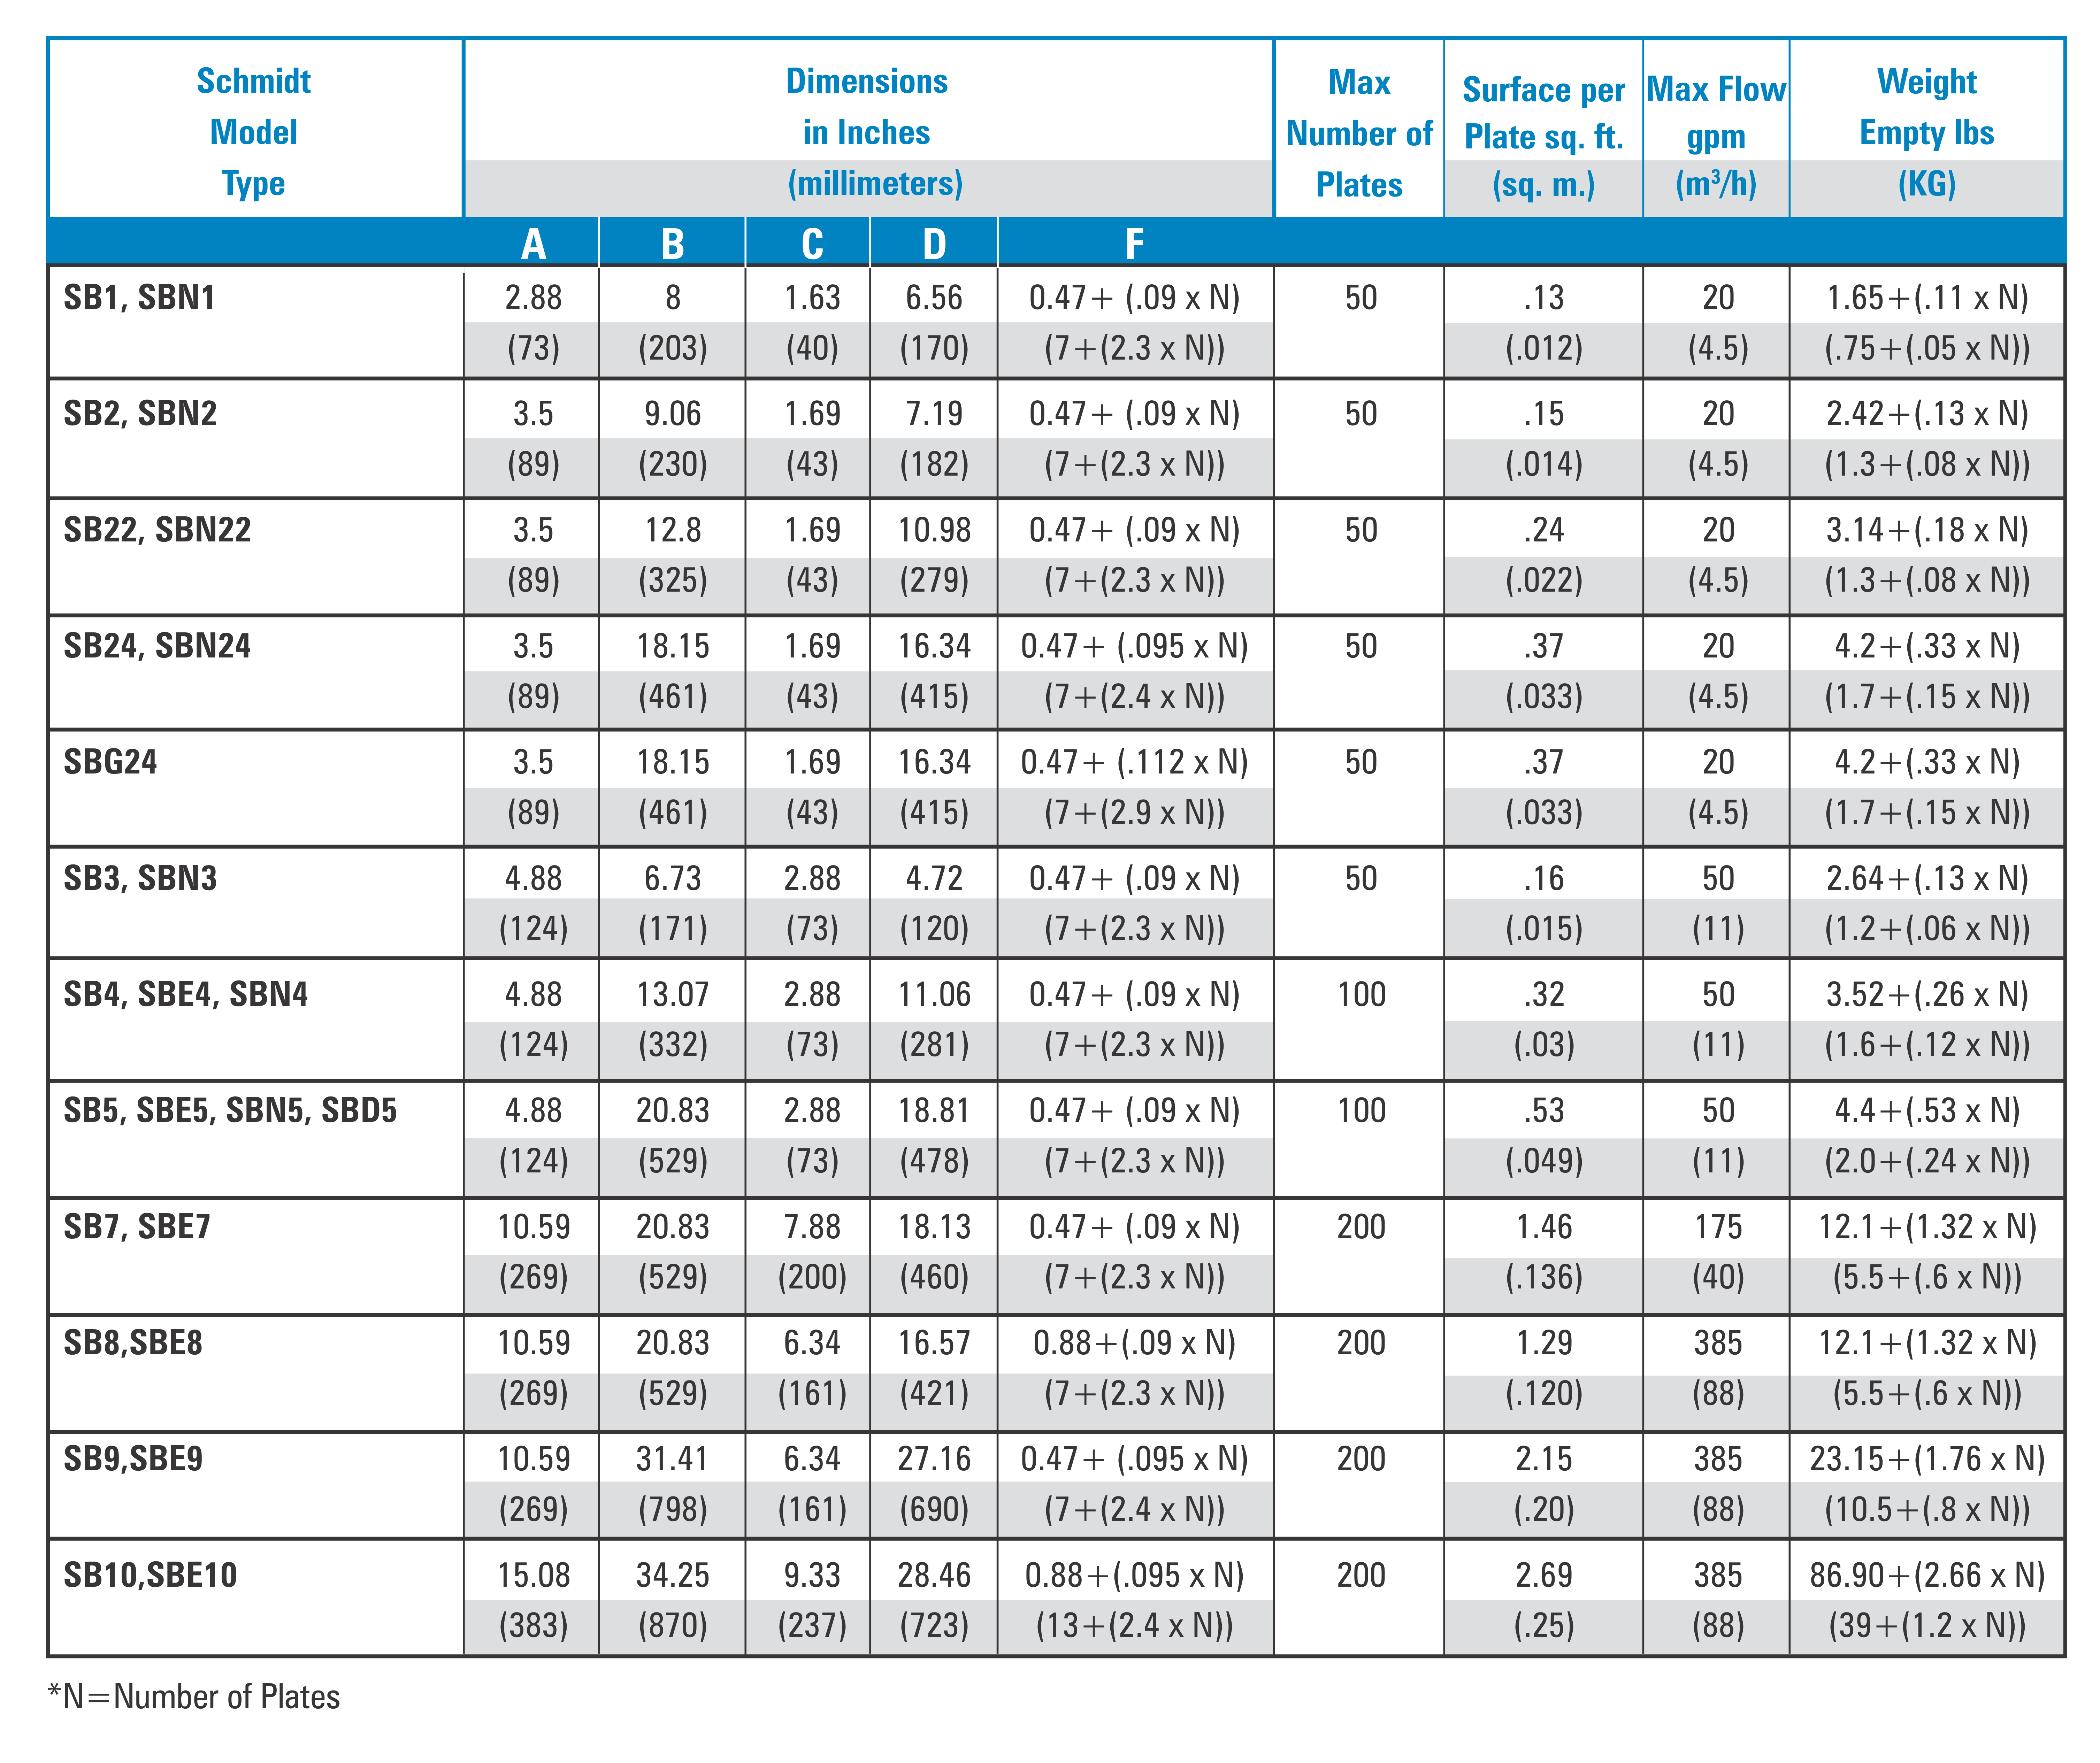
\includegraphics[width=5.0in]{schmidt_props.png}
\caption{Schmidt Brazed Heat Exchanger Properties}
\end{figure}

The average thickness of each plate may be roughly calculated as in equation \ref{eq:thickness}, where \(t_{\textrm{plate}}\) is the thickness of the plate, \(\Delta W\) is the change in weight per added plate, \(A_s\) is the surface area of one side of the plate, and \(\rho\) is the density of 316 stainless steel.

\begin{equation}
\label{eq:thickness}
t_{\textrm{plate}} = \frac{\Delta W}{\rho A_s}
\end{equation}

From this, the space between plates may also be calculated as in equation \ref{eq:spacing}, where \(\Delta l_z\) is the change in the depth of the heat exchanger per added plate.

\begin{equation}
\label{eq:spacing}
t_{\textrm{gap}} = \Delta l_z - t_{\textrm{plate}}
\end{equation}

The real-life plates are ribbed, which increases the convective heat transfer coefficients for heat transfer through the device. Unfortunately, finding these coefficients for such a complicated geometry would require computational fluid dynamics and heat transfer using a finite element method, which is out of the scope of this analysis.  Therefore, we will assume that the plates are flat, and know that the real-life convective heat transfer coefficients are significantly higher.

Assuming a flat plate, one may calculate the heat transfer coefficient using the empirical formula in equation \ref{eq:nukoverl}, where all physical properties are with respect to the fluid:

\begin{align}
\label{eq:nukoverl}
h &=\frac{k}{l} 0.037\textrm{Re}^{0.8}\textrm{Pr}^{1/3}\\
\label{eq:re}
\textrm{Re}&=\frac{\rho v t_{\textrm{gap}}}{\mu}\\
\label{eq:pr}
\textrm{Pr}&=\frac{\mu c_P}{k}
\end{align}

As mentioned previously, finding Re requires knowing the velocity of the fluids through the heat exchanger.  The volumetric flow rate of the hot fluid, in gallons per minute, is supplied, and may be used to find the average velocity through the heat exchanger through the relation in equation \ref{eq:flow2vel}.

\begin{equation}
\label{eq:flow2vel}
v = \frac{2\dot{V}}{l_x l_z}
\end{equation}

However, the volumetric flow rate for the building heating system is unknown. However, the flow rate necessary to meet the given design constraints may be calculated, from which the velocity for the cold side may be found in a similar manner. 

Due to the first law of thermodynamics and assuming adiabatic heat transfer (which I do throughout), equation \ref{eq:firstlaw} must be satisfied.

\begin{equation}
\label{eq:firstlaw}
\left(\dot{m} c_P \Delta T \right)_{\textrm{hot}} \left(\dot{m} c_P \Delta T \right)_{\textrm{cold}}
\end{equation}

Since all the \(\Delta T\)s are known, \(\dot{m}_{\textrm{hot}}\) may be calculated by dividing \(\dot{Q}_{\textrm{hot}}\) by \(\rho\), and \(c_P\) is a function of temperature, one may solve for \(\dot{m}_{\textrm{hot}}\), which may be converted back to \(\dot{Q}_{\textrm{cold}}\) and consequently to \(v\).

Referring back to equation \ref{eq:flow2vel}, notice that \(l_z\) is a function of \(N\), or the number of plates on the heat exchanger as can be seen in figure \ref{tab:schmidt}. This means that, ultimately, \(U\) and \(A_s\) are both functions of \(N\), and due to the functional nature of the material properties of the brines used, finding an analytical solution to this problem is nearly impossible.  Instead, this may be solved as a zero-finding problem. In other words, the \(N\) which satisfies this equation is the solution to equation \ref{eq:zeros}.

\begin{equation}
\label{eq:zeros}
0 = (UA_s)_{\textrm{required}} - U(N) A_s(N)
\end{equation}

Hence, given dimensions of a plate heat exchanger (with dimensions \(l_x\) and \(l_y\)) and the inlet and outlet temperatures of both the hot and the cold side, the number of plates required to achieve the required heat exchanger performance may be calculated.

\end{document}
